\documentclass{article}

% if you need to pass options to natbib, use, e.g.:
% \PassOptionsToPackage{numbers, compress}{natbib}
% before loading nips_2016
%
% to avoid loading the natbib package, add option nonatbib:
% \usepackage[nonatbib]{nips_2016}

\usepackage[final, nonatbib]{nips_2016}

% to compile a camera-ready version, add the [final] option, e.g.:
% \usepackage[final]{nips_2016}

\usepackage[utf8]{inputenc} % allow utf-8 input
\usepackage[T1]{fontenc}    % use 8-bit T1 fonts
\usepackage{hyperref}       % hyperlinks
\usepackage{url}            % simple URL typesetting
\usepackage{booktabs}       % professional-quality tables
\usepackage{amsfonts, amssymb, amsmath}       % blackboard math symbols
\usepackage{nicefrac}       % compact symbols for 1/2, etc.
\usepackage{microtype}      % microtypography
\usepackage{graphicx}
\usepackage{algpseudocode}
\usepackage{algorithmicx}
\usepackage{csvsimple}


\newcommand{\bX}{\mathbf{X}}
\newcommand{\bY}{\mathbf{Y}}
\newcommand{\bbeta}{\mathbf{\beta}}



\graphicspath{ {images/} }

\title{Survival of the Fittest: Variable Selection on Galapagos Agricultural Data}

\author{
  Michael Bostwick\\
  Department of Statistics and Operations Research\\
  University of North Carolina at Chapel Hill\\
  \texttt{mgb2188@live.unc.edu} \\
}


\begin{filecontents*}{scientists.csv}
name,surname,age
Albert,Einstein,133
Marie,Curie,145
Thomas,Edison,165
\end{filecontents*}

\begin{document}

\maketitle
\begin{abstract}
  This paper...
  
  \end{abstract}

\section{Introduction}

\subsection{Background}

The Galapagos Islands make for a feasible and significant case study of complex systems. Due to its relative isolation and smaller size the interaction of factors can more realistically be modeled for the Galapagos Islands than other systems. Yet the Galapagos Islands also represents an important example of the competing forces of resource conservation and economic development in a rapidly changing environment. Prior work has created agent-based models of the Galapagos, but with limited interaction parameters between agents, particularly in regards to farm success walsh. In order to create a more detailed, and perhaps more accurate, simulation, the relationships between different factors on the island must be better understood. This work aims to sort through a large number of possible relationships and clarify the empirically most significant ones for future study and incorporation into simulations. 

\subsection{Data}

The data available to study the dynamics between agricultural measures and related factors primarily 
comes from the Census of Agricultural Production Units (UPA) of Galapagos (Censo de las Unidades 
de Producci\'on Agropecuaria (upa) de Gal\'apagos). This is a self-reported survey with data from 755 
farms detailing the production and sale of crops and livestock, agricultural expenses, and land use 
decisions.

In addition to the census, data is also available from ... including information on water, energy and road access.

In total, under the direction of the client 240 variables were selected for consideration in modeling 
relationships between predictors and the outcome variables of interest.


\section{Modeling}
\subsection{Challenges to address}

The primary challenge in this analysis is the vast amount of potential predictor variables. This challenge is twofold; a.) when 
the number of predictors is large the calculation of a reliable model is difficult and b.) interpreting the coefficients of many 
predictors simultaneously is not an easy task for humans (and will make resulting simulations overly complicated). For this 
reason, the analysis focuses on the use of several variable selection techniques and a comparison of their performance. 
These variable selection techniques aim to build a linear model with a subset of the available variables that still maintains 
a strong predictive performance.

Secondarily, when performing standard linear regression the outcome variable is assumed to be roughly normally 
distributed. When this is not true, as is the case for several outcome variables in this study, a poorly fitting model will be 
found with unreliable coefficients. In order to address this issue transformations to the data and modifications to the 
standard linear model will be considered.

\subsection{Overview of methods}

A brief overview of the statistical methods used is presented here to allow for understanding of results, 
but for further details see Section refstatmethods Statistical Methods. For each of the outcome variables of interest 
we build a set of linear models using the appropriate subset of predictors. Each relationship is modeled 
using Best Subset, Forward Selection and ElasticNet regression. Best Subset considers all variable combinations to find the 
linear model of best fit. Forward Selection fits a linear model by progressively adding variables to the model until a best fit is 
found. This results in only some of the variables being included, chosen in a discrete manner. ElasticNet regression fits a linear 
model by constraining the coefficients so that they are smaller than in standard least squares, and for many variables actually 
shrunken to zero. Similar to Forward Selection this results in a sparser model, but variable selection can be carefully tuned 
as optimization is done in a more continuous way.

\section{Results}

\subsection{Farm Success}

We define farm success with three different measurements: productivity, net income and number of workers supported. Productivity is calculated as the total pounds of crops and livestock produced divided by the farm surface area. Net income is calculated as the difference between the earnings from all products sold and total expenses. Number of workers supported is calculated as the total labor expenditures divided by a standard worker's salary.

\subsubsection{Productivity}

Response variable plots and discussion
\begin{figure}[h]
\centering
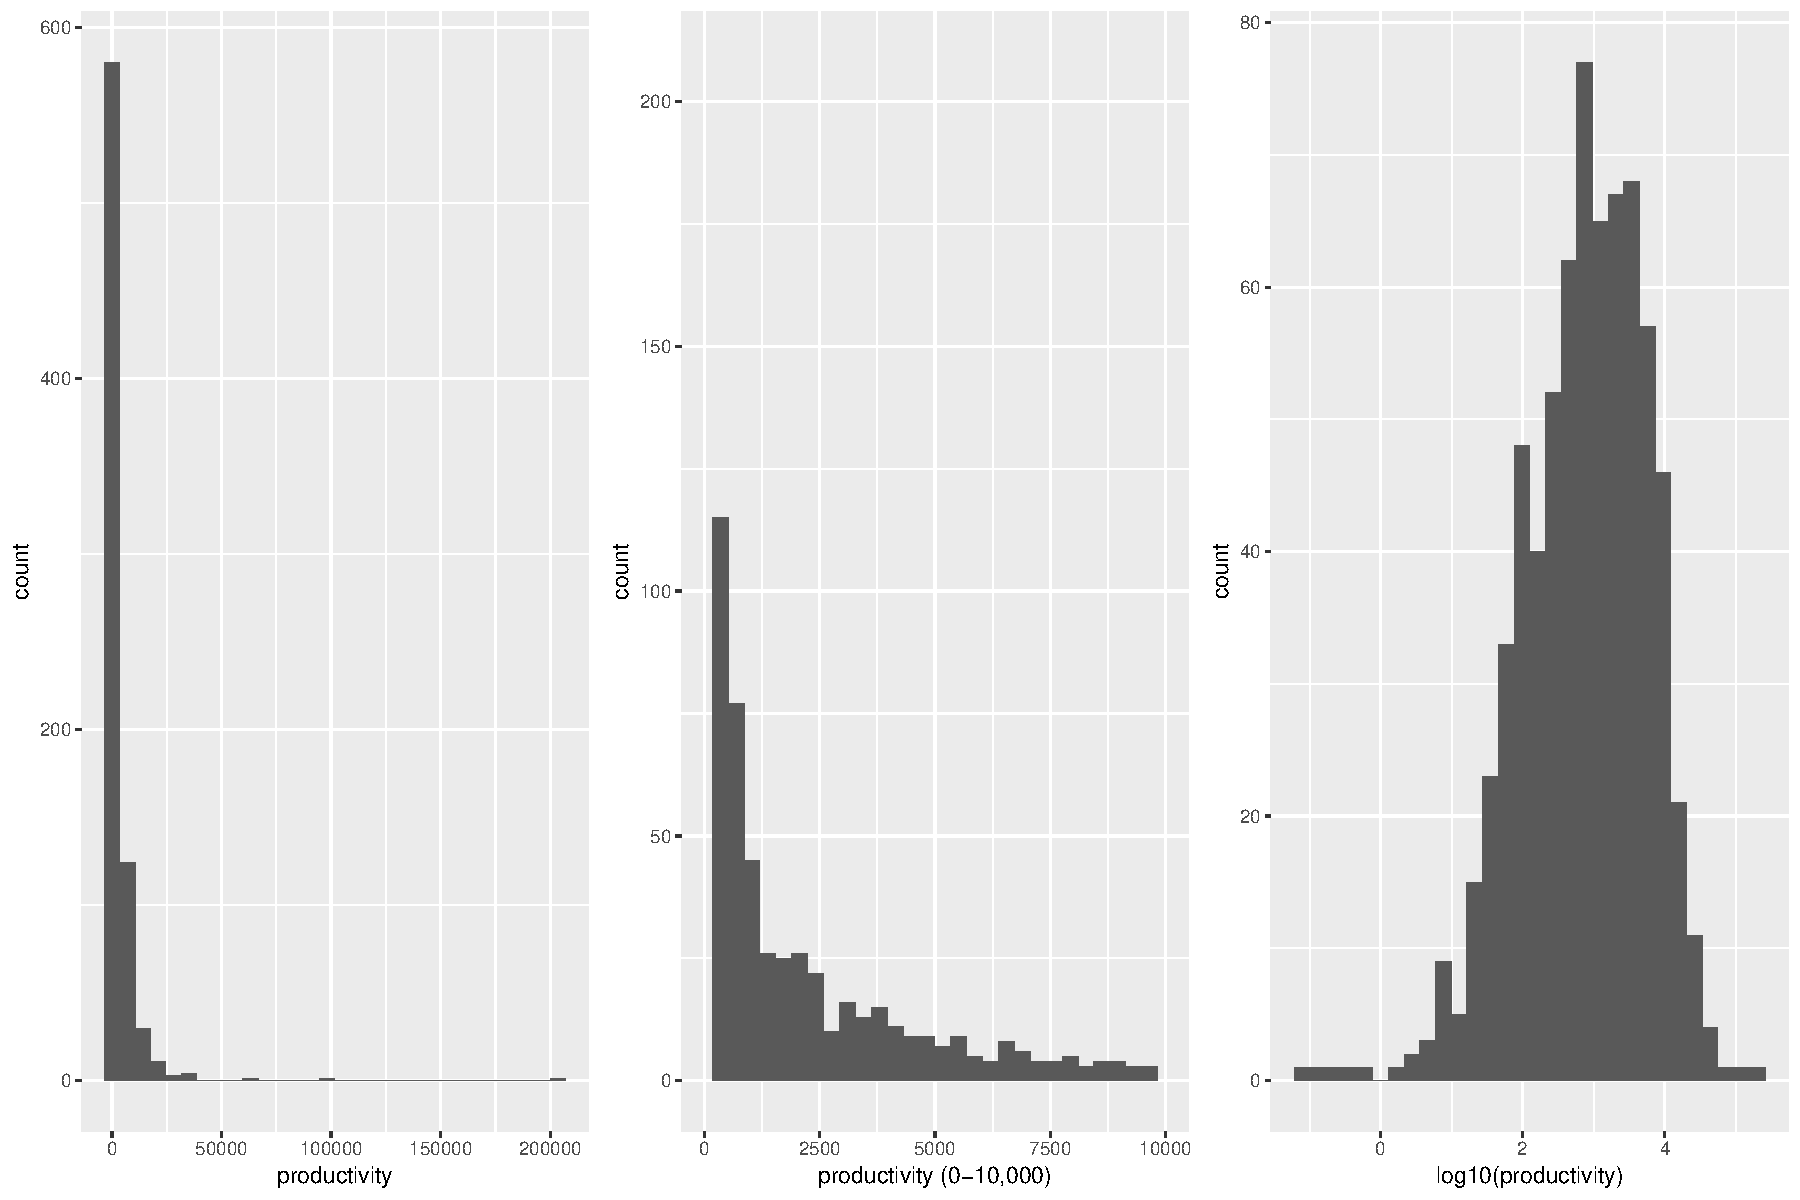
\includegraphics[width = 0.75\textwidth]{production_histograms.pdf}
\caption{Histogram of Productivity...}
\end{figure}


\begin{table}[h!]
\centering
\begin{tabular}{c|c|c}\hline%
\bfseries \underline{Elasticnet} & \bfseries \underline{Forward~Selection} & \bfseries \underline{Best~Subset}
\csvreader[head to column names]{production_top10names.csv}{}%
{\\\elasticnet & \forward & \subset}%
\\\hline
\end{tabular}
\caption{Modeling of Productivity, Top 5 features for each of the three methods}
\label{table:1}
\end{table}


\begin{figure}
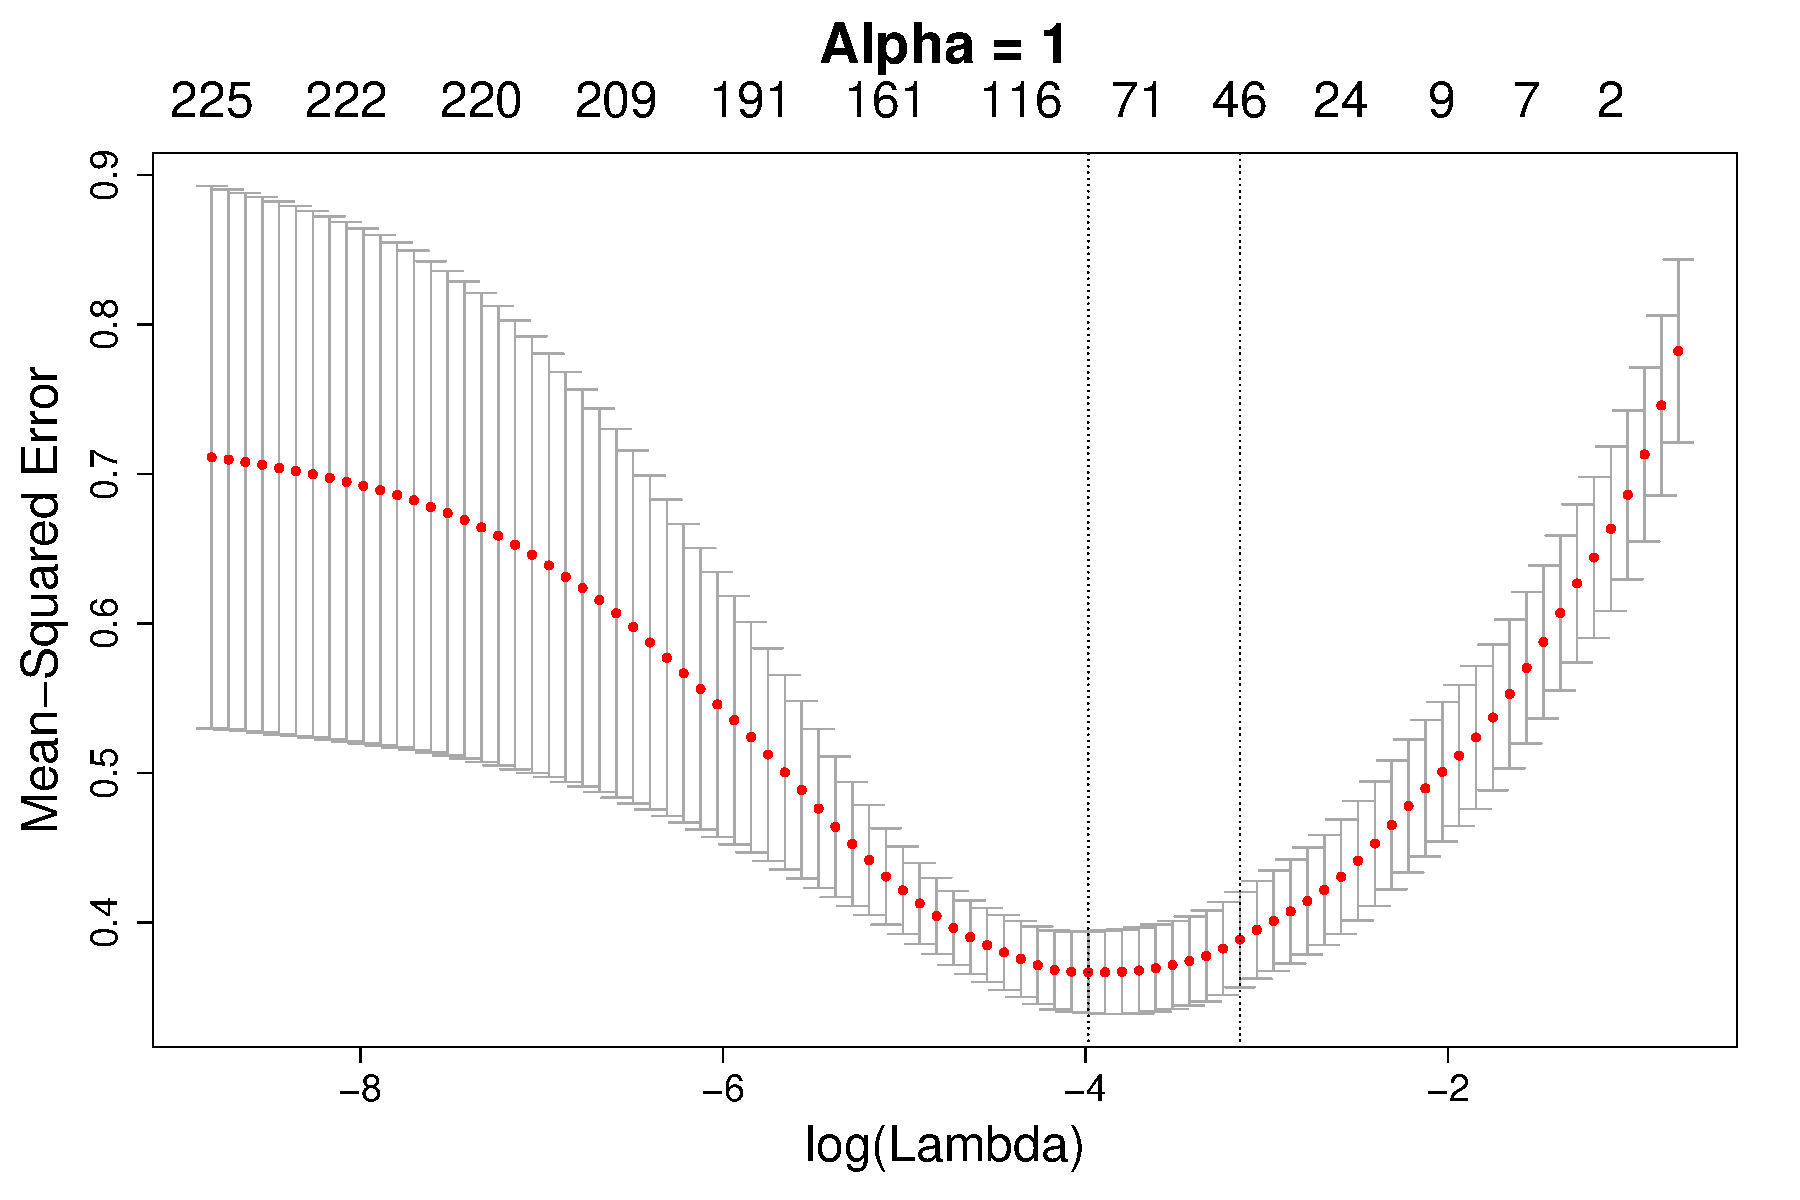
\includegraphics[width = \textwidth]{elastic_cv_production.pdf}
\caption{Cross Validation plots for Elasticnet...}
\end{figure}

\begin{figure}
\centering
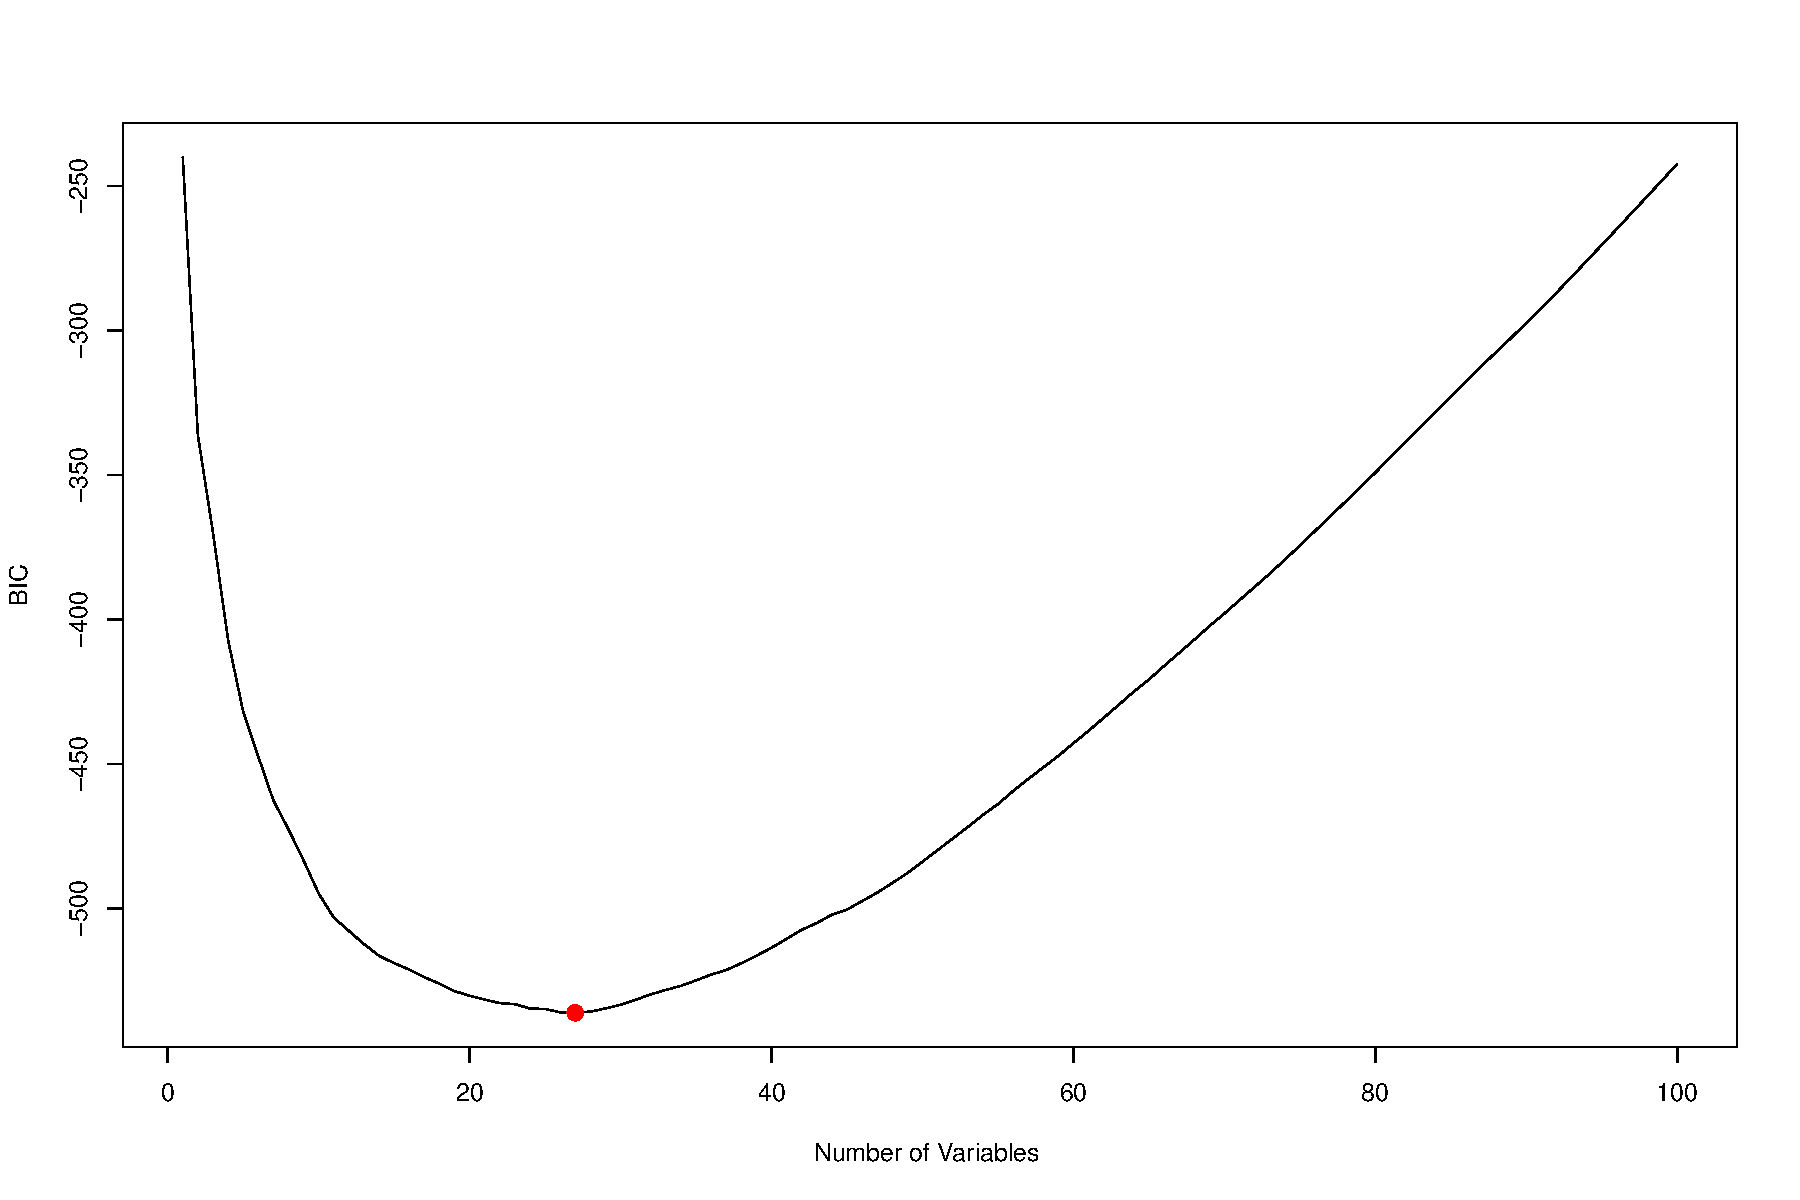
\includegraphics[width = 0.8\textwidth]{forward_nvars_production.pdf}
\caption{Number of variables Forward Selection plots...}
\end{figure}

Bootstrap plots

\subsubsection{Net Income}

\begin{figure}[h]
\centering
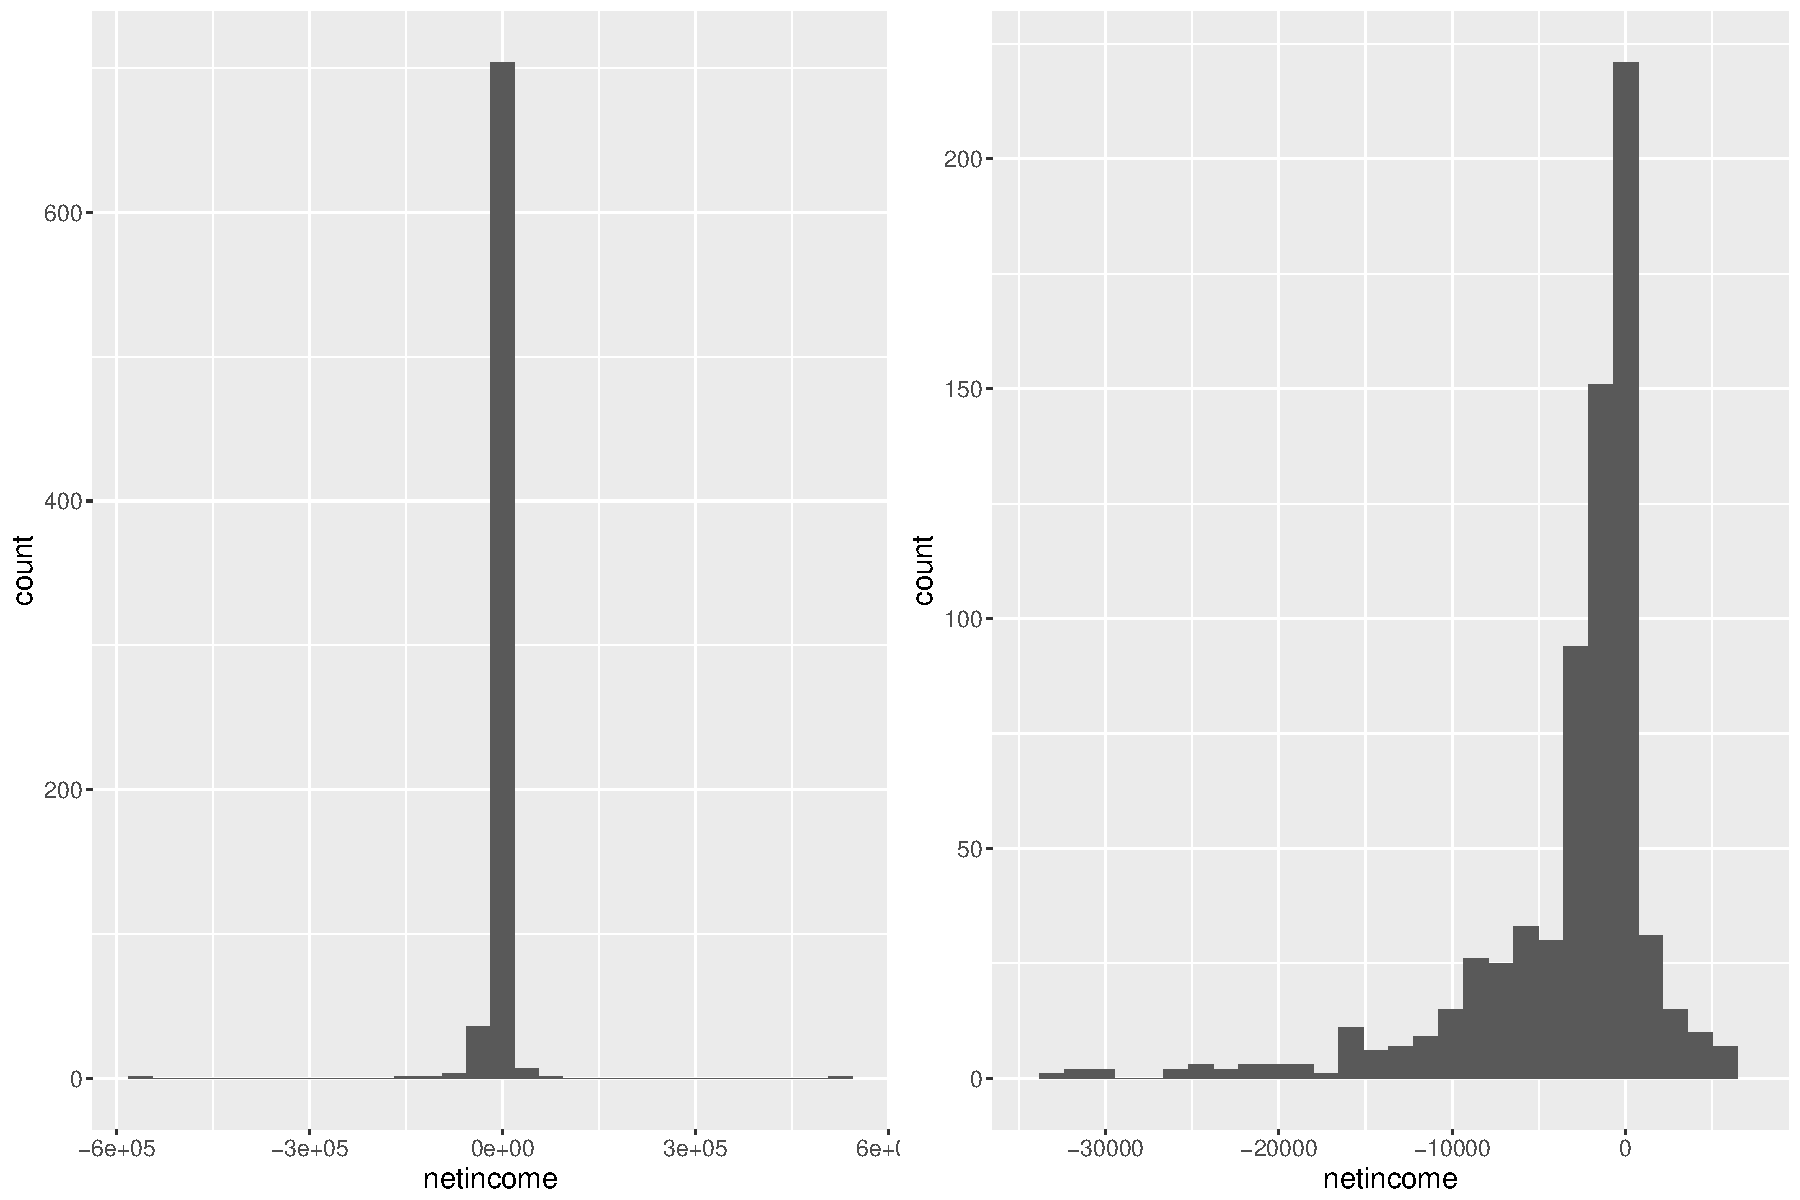
\includegraphics[width = 0.75\textwidth]{netincome_histograms.pdf}
\caption{Histogram of Net Income...}
\end{figure}


\begin{table}[h!]
\centering
\begin{tabular}{c|c|c}\hline%
\bfseries \underline{Elasticnet} & \bfseries \underline{Forward~Selection} & \bfseries \underline{Best~Subset}
\csvreader[head to column names]{netincome_top10names.csv}{}%
{\\\elasticnet & \forward & \subset}%
\\\hline
\end{tabular}
\caption{Modeling of Net Income, Top 5 features for each of the three methods}
\label{table:1}
\end{table}


\begin{figure}
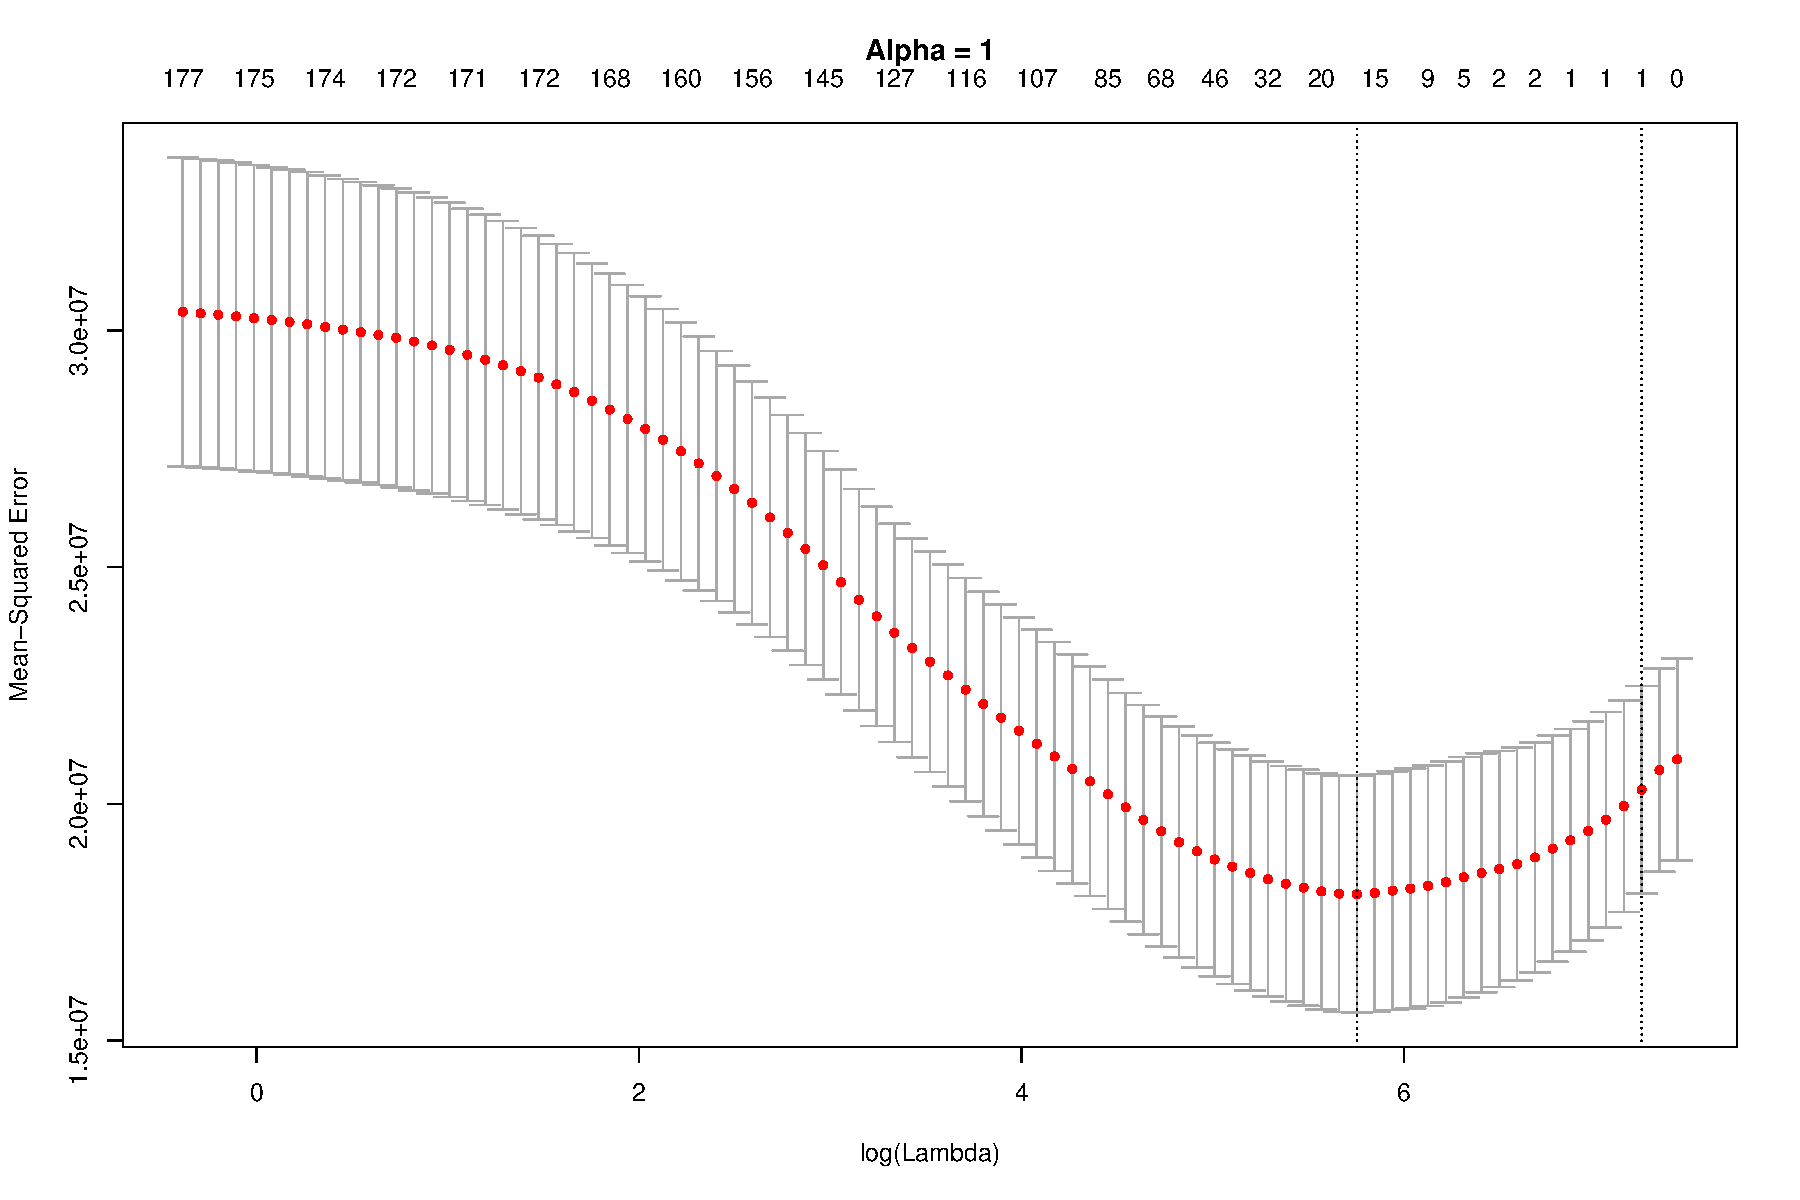
\includegraphics[width = \textwidth]{elastic_cv_netincome.pdf}
\caption{Cross Validation plots for Elasticnet...}
\end{figure}

\begin{figure}
\centering
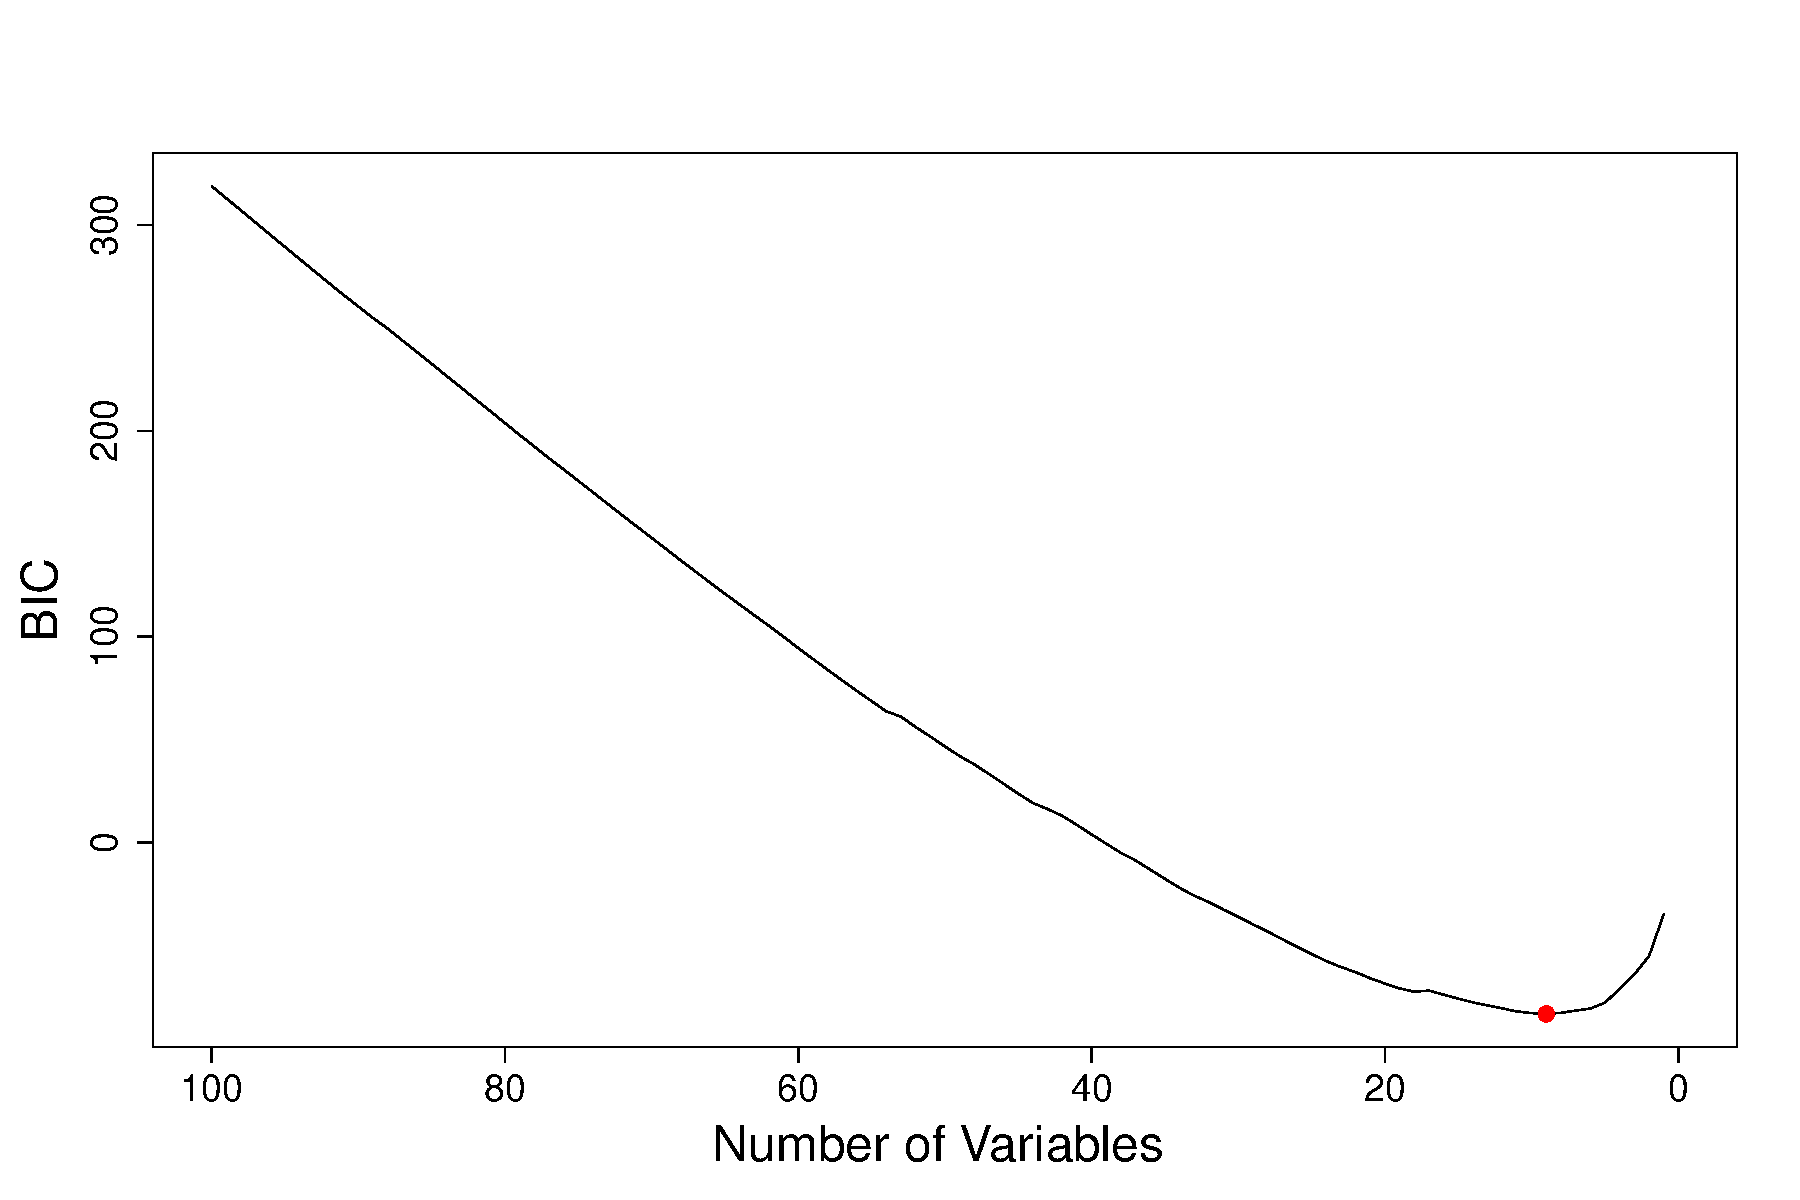
\includegraphics[width = 0.8\textwidth]{forward_nvars_netincome.pdf}
\caption{Number of variables Forward Selection plots...}
\end{figure}


\subsubsection{Number of Workers Supported}


\subsection{Invasive Species}

\subsection{Land use choices}


\section{Statistical Methods} \label{stat_methods}

\subsection{Generalized Linear Models}

\[\bY = \bX\beta + \epsilon \tag{1}\]
%\[Y_i =  \sum_{j=1}^{p} X_{i,j}\beta_j + \epsilon \tag{1}\]

Standard Linear Regression can be represented in matrix form as equation 1 above, where $\bY$ is a $n \times 1$ vector of 
the outcome variable, $\bX$ is a $n \times p$ matrix of the predictor variables, $\bbeta$ is a $p \times 1$ vector of variable coefficients and $\epsilon$ is the error 
term. The standard linear model assumes the outcome variable $\bY$ has a normal distribution, and therefore takes 
continuous values. When the outcome variable is continuous, but not normal shaped (perhaps skewed like the productivity 
data) it can be possible to transform the data by taking the logarithm or something similar. However, when the outcome 
variable is discrete (such as labels of 1 and 0 denoting absence/presence of agricultural land use) a further modification must be made. The outcome variable is clearly no longer normally distributed, as it is not even continuous. Without modification we could get predicted values below 0, above 1 or somewhere in between, none of which make much sense.

This calls for the use of logistic regression, in which we perform a logit transformation as seen in the equation below so that the 
$\bX\beta$ can still be mapped to a continuous scale. In some respects this is a computational concern, but it also changes the 
way coefficients can be interpreted. Instead of a one unit change in $X_1$ predicting a $\beta_1$ change in the predicted $Y$, 
in this case it predicts a $\beta_1$ change in the log odds of $Y$.

\[log \frac{\Pr(Y = 1)}{\Pr(Y = 0)} = \bX\beta \]

This equation can be rewritten as below

\[ \Pr(Y = 1) = \frac{e^{\bX\beta}}{1 + e^{\bX\beta}} \]

Multiclass Logistic Regression

\[ \Pr(Y = k) = \frac{e^{\bX\beta_k}}{\sum_{l=1}^{K-1} e^{\bX\beta_l}} \]

% include Poisson function

\subsection{Performance Measures}

There are many measures of the fit of linear models. Since there are many possible predictor variables, care must be taken 
to use appropriate measures, as some measures will favor just adding all of the variables to the model. For example, if we 
aim to minimize the mean square error adding more predictor variables to the model will always be encouraged. Since that is not desired, measurements like Bayesian Information Criterion (BIC) and Mallow's $C_p$ ($C_p$) can used here. BIC and $C_p$ are a combination of how well the model fits the data and a penalty term for the number of predictor variables included in the model. The goal is to minimize BIC and $C_p$, that is the model with the best balance of small size and goodness of fit. BIC puts a large penalty on the inclusion of additional variables, so it will be our primary metric.

Another approach is to use cross-validation. In this technique the dataset is first split into $n$ equally sized sets. Then a 
model is fit using $n - 1$ of the sets (training sets) and evaluated on the remaining 1 (test) set. This is repeated $n$ times, 
each time reserving a different 1 test set, and then results across the $n$ runs are averaged. The benefit of this is that model 
building and model evaluating are happening on different portions of the data, so we can distinguish if the model is picking up 
on generalizable patterns or just random noise. Using cross-validation the average test set mean square error is an 
appropriate measure of model fit.

\subsection{Best Subset and Forward Selection}

The essential goal of variable selection is to find the best combination of predictor variables to explain the outcome variable. As 
discussed above, when we have many possible predictors we often want to put a constraint on the problem so that all variables 
are not included. Such a constraint might be limiting the number of variables included or that the model found can generalize to 
other data. Best subset selection, the most natural, but computationally difficult way is to try all possible combinations of variables and select the best fitting combination. However, when the number of variables, $p$, is large this quickly becomes infeasible, as there are $2^p$ possible combinations. Recent advances have expanded the problem sizes that can be efficiently computed using Mixed Integer Optimization. Using this technique we find the best 5 variable models for each of the outcomes, but are not able to search all possible model sizes to find the optimal number of variables. In addition, as marked in the results above, sometimes the algorithm can verify that it has found the optimal solution, while other times it returns the best solution found in the allotted time limit (set to 60 seconds), that may or may not be the overall optimal solution.

One approach to tackle the computational complexity discussed above is to restrict the search for the optimal number of 
predictor variables, which is what Forward Selection does. In this algorithm, we start with an empty model and iteratively add a 
new variable at each stage that is most beneficial. This procedure can work well, but may not find the optimal solution. As an example, consider a case where $X_1$ is the single most predictive variable, but the combination of $X_2$ and $X_3$ is the best two variable combination. The algorithm will first add $X_1$, but then regardless whether it adds $X_2$ or $X_3$ next, it will have found a suboptimal solution. In general, we can decide to stop adding variables once we have reached an optimal performance measure like BIC or cross-validation test error.


\subsection{Regularized Regression}

% Consider taking these out of matrix form

	\[\min_{\beta}  \|\bY - \bX\beta\|_{2}^{2} \tag{linear model}\]
	\[\min_{\beta}  \|\bY - \bX\beta\|_{2}^{2} + \lambda||\beta||_2^2 \tag{ridge regression}\]
	\[\min_{\beta}  \|\bY - \bX\beta\|_{2}^{2} + \lambda||\beta|| \tag{LASSO}\]

As shown in equation ? in the standard linear model, we try to find the $\beta$ that minimizes the squared difference between 
the true $\bY$ and the predicted $\hat{\bY}$ (which is $\beta\bX$). In regularized regression we do the same thing, but also 
add a second term that we look to simultaneously minimize. This second term adds a penalty for increasing values of $
\beta$, so the two terms must be balanced. The optimal model will find a balance between fitting the outcome variable 
closely, but not having too large of coefficient values. The difference between Ridge regression and LASSO is how we add up 
the coefficients. In Ridge Regression the coefficients are squared and then summed, in LASSO we take the absolute value of 
the coefficients and then sum them. LASSO will encourage most of the coefficients to go to zero, thus only including a small 
number of terms in the model. Ridge regression will encourage the coefficient values to be spread out among predictor 
variables, leaving all of the variables in the model, but helping to offset negative effects of correlated predictor variables. Further explanations of this can be found in ???

\[\min_{\beta}  \|\bY - \bX\beta\|_{2}^{2} + \lambda[(1 - \alpha)||\beta||_2^2 + \alpha||\beta||] \tag{ElasticNet}\]

The technique that is used in this analysis is a combination of the Ridge and LASSO penalties, called ElasticNet. As can be seen in the equation above both the square of the coefficients and the absolute value of the coefficients is included, with the contribution of each controlled by the size of $\alpha$ which takes a value between 0 and 1. ElasticNet, thus combines the favorable properties of Ridge and LASSO in that it can achieve both sparse models and deal with correlated predictor variables. Both the $\lambda$ and the $\alpha$ can be set using cross-validation (as discussed above) to be appropriate values for the particular dataset. 

\subsection{Comparison of methods}


\section{Conclusion}


\medskip

\small

\begin{thebibliography}{99}




\end{thebibliography}

\section{Appendix}

\begin{table}[h!]
\begin{tabular}{l|c|c}\hline%
\bfseries \underline{Variable} & \bfseries \underline{Elasticnet} & \bfseries \underline{Forward~Selection}
\csvreader[head to column names]{fullcoeflist_production.csv}{}%
{\\\variable & \elastic & \forward}%
\\\hline
\end{tabular}
\caption{Full coefficient list for Production model}
\end{table}

\begin{table}[h!]
\begin{tabular}{l|c|c}\hline%
\bfseries \underline{Variable} & \bfseries \underline{Elasticnet} & \bfseries \underline{Forward~Selection}
\csvreader[head to column names]{fullcoeflist_netincome.csv}{}%
{\\\variable & \elastic & \forward}%
\\\hline
\end{tabular}
\caption{Full coefficient list for Net Income model}
\end{table}

\begin{figure}[h]
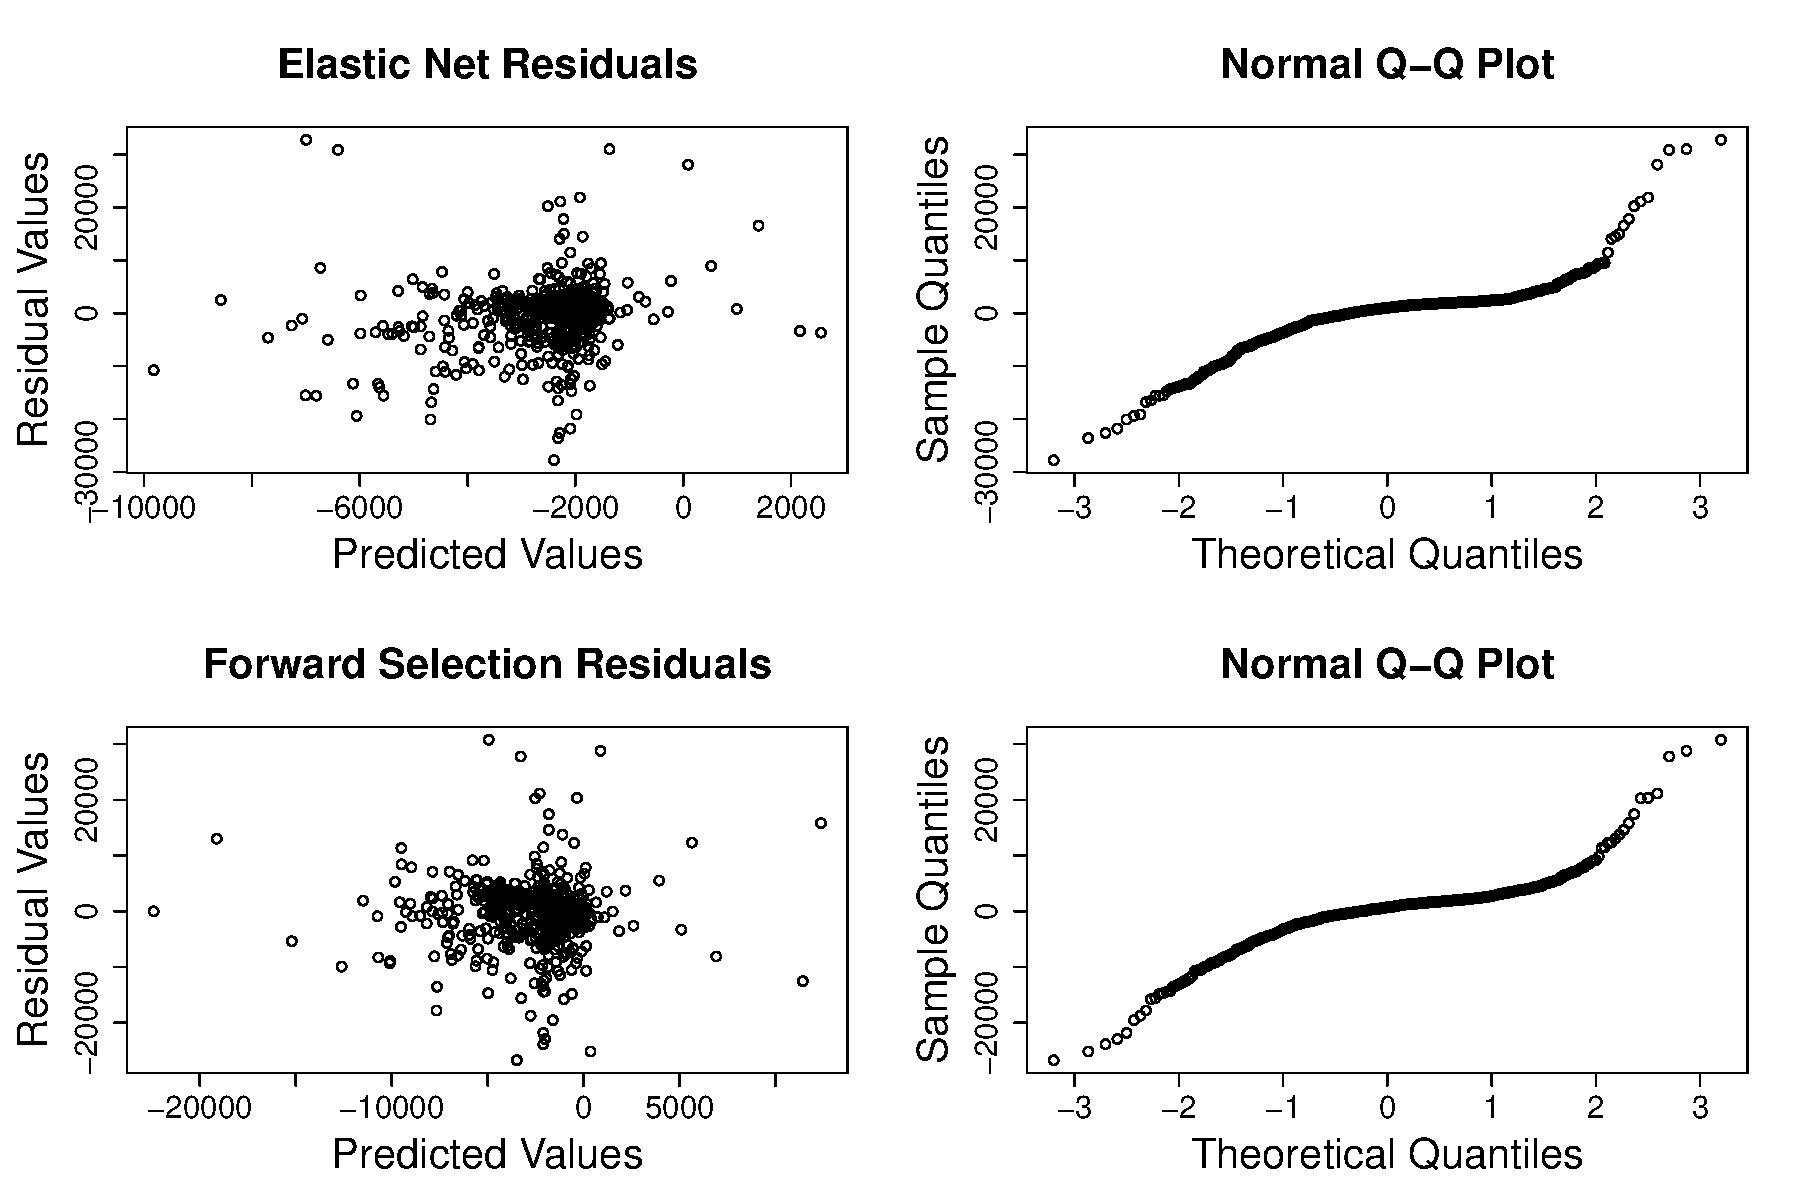
\includegraphics[width = \textwidth]{resids_netincome.pdf}
\caption{Diagnostic Residual plots for Net Income...}
\end{figure}

\end{document}



